\RCS$Revision$
\RCS$HeadURL$
\RCS$Id$
\newlength\cmsFigWidth

\ifthenelse{\boolean{cms@external}}{\setlength\cmsFigWidth{0.98\columnwidth}}{\setlength\cmsFigWidth{0.69\textwidth}}
\ifthenelse{\boolean{cms@external}}{\providecommand{\cmsLeft}{top\xspace}}{\providecommand{\cmsLeft}{left\xspace}}
\ifthenelse{\boolean{cms@external}}{\providecommand{\cmsRight}{bottom\xspace}}{\providecommand{\cmsRight}{right\xspace}}

\newcommand{\sqrts}{ \ensuremath{\sqrt{s}}\xspace}
\newcommand{\RAA}{\ensuremath{R_{\mathrm{AA}}}\xspace}
\newcommand{\TAA}{\ensuremath{T_{\mathrm{AA}}}\xspace}
\newcommand{\PbPb}{\ensuremath{\mathrm{PbPb}}\xspace}
\newcommand{\pp}{\Pp{}\Pp}
\newcommand{\pPb}{\Pp{}\ensuremath{\mathrm{Pb}}\xspace} %check
\newlength\cmsTabSkip\setlength{\cmsTabSkip}{1ex}
\providecommand{\Pphi}{\PGfP{1020}}
\providecommand{\PABzs}{\ensuremath{\overline{\PBzs}}\xspace}
%\newcommand{\Bplusdecay}{\ensuremath{\PBp\rightarrow\PJGy\,\PKp}\xspace}
%\newcommand{\Bzerodecay}{\ensuremath{\cmsSymbolFace{B}^{0}\rightarrow \PJGy~\PK^{*}(892)^{0}}\xspace}
%\newcommand{\Bzerosdecay}{\ensuremath{\PBzs\rightarrow\PJGy\,\Pphi}\xspace}
\providecommand{\Bzerosdecayall}{\ensuremath{\PBzs \to \PJGy\Pphi \to \Pgmp\Pgmm\PKp\PKm}\xspace}
\providecommand{\Bplusdecayall}{\ensuremath{\PBp \to \PJGy\PKp \to \Pgmp\Pgmm\PKp}\xspace}
\providecommand{\Bzerosdecay}{\ensuremath{\PBzs \to \PJGy\Pphi}\xspace}
\providecommand{\Bplusdecay}{\ensuremath{\PBp \to \PJGy \PKp}\xspace}
\newcommand{\Jpsidecay}{\ensuremath{\PJGy\rightarrow\PGmp\PGmm}\xspace}
\newcommand{\dstardecay}{\ensuremath{\PDst \rightarrow \PK \PGp\PGp(\PGp\PGp)\xspace}}
\newcommand{\phidecay}{\ensuremath{\Pphi\rightarrow \PKp \PKm \xspace}}
\providecommand{\HYDJET}{\textsc{hydjet}\xspace}
\providecommand{\NA}{\ensuremath{\text{---}}}
\newcommand{\npart}{\ensuremath{\langle N_{\text{part}}\rangle}\xspace}
\newcommand{\NMB}{\ensuremath{N_{\text{MB}}}}


%\newcommand{\comment}[1]{{\color{red} $\leadsto$ #1}}
\newcommand{\comment}[1]{{}}


\cmsNoteHeader{HIN-19-011}

\title{Measurement of B$_s^0$ and B$^+$ meson yields in PbPb collisions at ${\sqrt{s_{\text{NN}}}} = 5.02$ TeV}

\address[cern]{CERN}
\author[cern]{The CMS Collaboration}

\date{\today}

\abstract{
The B$^{0}_s$  and B$^{+}$  production cross sections are measured in lead-lead (PbPb) collisions at a center-of-mass energy per nucleon pair of 5.02\,TeV.
The data sample, collected with the CMS detector at the LHC, corresponds to an integrated luminosity of $1.7\,\text{nb}^{-1}$.
The mesons are reconstructed in the exclusive decay channels B$^{0}_s\rightarrow{J}/\psi\,\phi(1020)$ and B$^{+}\rightarrow{J}/\psi\,K^{+}$ where the ${J}/\psi$ ($\phi$(1020)) meson is $\mu^{+}\mu^{-}$ ($K^{+}K^{-}$)
%within the rapidity range $\abs{y}<2.4$.
The B$^{0}_s$ meson is observed with a statistical significance in excess of fivef standard deviations for the first time in nucleus-nucleus collisions.
The measurements are performed as a function of the transverse momentum of the B mesons, in the interval 7--50\,GeV$/c$, % for ${B}^{+}$ (${B}^{0}_s$), 
and of the PbPb collision centrality.
The ratio of production yields of {B}$^{0}_s$  and {B}$^{+}$ is also presented. 
%The ratio shows hints of a $p_\text{T}$ dependence, decreasing from low- to high-$p_\text{T}$, and no significant centrality dependence is observed.
}


\hypersetup{%
pdfauthor={N. Leonardo, Z. Shi, G.-J. Kim, J. Silva, A. Pardal, J. Goncalves, J. Wang, C. Mironov, Y.-J. Lee; CCLE: M. Nguyen},%
pdftitle={Measurement of Bs and B+ meson production cross sections in PbPb collisions at 5.02 TeV},%
pdfsubject={CMS},%
pdfkeywords={physics, quark gluon plasma, heavy flavor, B meson}}

\maketitle

\section{Introduction}

Relativistic heavy ion collisions allow the study of quantum chromodynamics (QCD) at high energy density and temperature. Under such extreme conditions, a state in which the quarks and gluons are the relevant degrees of freedom, the quark-gluon plasma (QGP)~\cite{QGP1,QGP2}, is predicted by the lattice QCD calculations~\cite{Karsch:2003jg}.
%
Multiple probes are necessary for characterizing the properties of the QGP medium created in heavy ion collisions and for thereby gaining further understanding of the underlying processes.
%
Heavy quarks are abundantly produced at the CERN Large Hadron Collider (LHC), and their exploration has the potential of providing novel insights in perturbative QCD calculations~\cite{Andronic:2015wma} and as probes of the QGP~\cite{Dong:2019byy}.
%
Hard-scattered partons lose energy by means of elastic collisions and medium-induced gluon radiation~\cite{Eloss1,Baier:2000mf,Chatrchyan:2011sx,Aad:2010bu,Andronic:2015wma} as they traverse the QGP.
The study of the phenomenon of parton energy loss can provide insights into the energy density and diffusion properties of the QGP.
%
The measurement of exclusive beauty and charm hadron decays facilitates added precision and allows the study of flavor and mass dependence for such processes. 
%
Although precise heavy flavor data became available at the BNL RHIC and the LHC, there are still large theoretical uncertainties on the hadronization of heavy quarks in the presence of QGP~\cite{Rapp:2018qla}. Therefore, a more precise understanding of the hadronization mechanism using fully reconstructed heavy-flavor mesons is needed for the extraction of transport properties of the QGP using heavy quarks. 

An enhancement in strangeness content~\cite{ALICE:2017jyt,Abelev:2013xaa,Agakishiev:2011ar,Abelev:2008zk,Arsene:2009jg,Adamczyk:2017wsl,Adare:2015ema} is expected when the medium temperature lies above the strange quark mass ~\cite{PhysRevLett.48.1066}. Complementary to the direct reconstruction of (light-quark) strange mesons and baryons, %it was suggested that the
strangeness content enhancement in the QGP may be further probed using heavy quarks.
%
Through a quark-recombination mechanism~\cite{Molnar:2003ff,Greco:2003mm,Greco:2003vf,Andronic:2015wma,He:2014cla}, a corresponding yield enhancement of hadrons containing strangeness is expected relative to corresponding hadrons that do not contain strange quarks. 
%
Hints of the presence of such recombination processes also for heavy mesons were recently detected in the open-charm~\cite{Acharya:2018hre} and open-beauty~\cite{BsPbPbCMS} sectors at the LHC, in lead-lead (\PbPb\) collisions at $\sqrtsNN=5.02\TeV$. 
%Because of the limited size of the available data samples, no definitive picture could be achieved.

The production of \PB\ mesons employing fully reconstructed decay was studied at the LHC in proton-proton (\pp\ ) collisions at center-of-mass energies of $\sqrts = 7\TeV$~\cite{CMSBmesonpp,Chatrchyan:2011pw,Chatrchyan:2011vh,ATLAS:2013cia,LHCb:2013JHEP,Aaij:2014hla,Aaij:2012dd}, 8\TeV~\cite{Aaij:2015fea,Aaij:2014ija} and 13\TeV~\cite{Khachatryan:2016csy} over wide transverse momentum (\pt) and rapidity ($y$) intervals, and in proton-lead ($\pPb$) collisions at a center-of-mass energy per nucleon pair of $\sqrtsNN = 5.02$\TeV~\cite{Khachatryan:2015uja}. In \PbPb collisions, the CMS Collaboration reported results at $\sqrtsNN = 5.02$\TeV for the \PBp~\cite{BpPbPbCMS} and \PBzs~\cite{BsPbPbCMS} mesons.
%
In this Letter, we extend these results, employing the \PbPb\ data set collected at the end of 2018, a sample larger by about a factor of three compared to the first measurement with 2015 data, resulting in increased statistical precision and significance.  

%The \PB\ mesons are measured in the interval $\abs{y}<2.4$ and $5<\pt<60\GeVc$,  via the fully reconstructed decay channels \Bzerosdecay\ and \Bplusdecay\, with \Jpsidecay\ and \phidecay.
The \PB\ mesons are reconstructed via the exclusive decay channels \Bzerosdecay\ and \Bplusdecay, with \Jpsidecay\ and \phidecay.
Throughout the paper, unless otherwise specified, the $y$ and \pt\ variables given are those of the $\PB$ mesons, and charge-conjugated states are assumed. The production cross sections of the \PBzs\ and \PBp\ mesons in \PbPb\ collisions at $\sqrtsNN = 5.02$\TeV and their ratios are reported here, using a data set corresponding to an integrated luminosity of 1.7\nbinv\ collected by the CMS experiment.
The measurements are performed as functions of the meson \pt and of the \PbPb collision centrality (which characterizes the degree of overlap of the two lead nuclei).
%which is related to the impact parameter of the two lead nuclei. 

\section{Experimental apparatus and data sample}

The central feature of the CMS detector is a superconducting solenoid, which provides a magnetic field of 3.8\unit{T}. Within the solenoid volume are a silicon tracker that measures charged particles in the pseudorapidity range $\abs{\eta} < 2.5$, a lead tungstate crystal electromagnetic calorimeter, and a brass and scintillator hadron calorimeter. For charged particles of $1 < \pt < 10$\GeVc and $\abs{\eta} < 1.4$, the track resolutions are typically 1.5\% in \pt and 25--90 (45--150)\mum in the transverse (longitudinal) impact parameter \cite{TRK-11-001}. Muons are measured in the range $\abs{\eta} < 2.4$, with detection planes made using three technologies: drift tubes, cathode strip chambers, and resistive-plate chambers. The muon reconstruction algorithm starts by finding tracks in the muon detectors, which are then fitted together with tracks reconstructed in the silicon tracker to form "global muons". Matching muons to tracks measured in the silicon tracker results in a relative \pt resolution for muons with $20 < \pt < 100$\GeVc of 1.3--2.0\% in the barrel and better than 6\% in the endcaps.
%For muons with higher \pt up to 1\TeVc, the \pt resolution in the barrel is better than 10\%~\cite{Chatrchyan:2012xi}.
The hadron forward (HF) calorimeter uses steel as an absorber and quartz fibers as the sensitive material. The two halves of the HF are located 11.2\unit{m} away from the interaction point, one on each end, providing together coverage in the range $3.0 < \abs{\eta} < 5.2$. In this analysis, the HF information is used to select \PbPb\ collision events and to define their centrality class. Centrality, defined as the fraction of the total inelastic hadronic cross section with 0\% representing collisions with the largest overlap of the two nuclei, is determined experimentally using the total energy in both HF calorimeters~\cite{centralityref}. 
%
Events are filtered using a two-tiered trigger system~\cite{Khachatryan:2016bia}. 
The first level (L1), composed of custom hardware processors, uses information from the calorimeters and muon detectors to select events within a fixed time interval of less than 4\mus. The second level, known as the high-level trigger (HLT), consists of a farm of processors running a version of the full event reconstruction software optimized for fast processing.
%
A detailed description of the CMS experiment and coordinate system can be found in Ref.~\cite{bib_CMS}.

Several Monte Carlo (MC) simulated event samples are used to evaluate background components, signal efficiencies and detector acceptance corrections. The simulations include samples containing only the $\PB$ meson decay channels being measured, and samples with prompt and nonprompt \PJGy mesons (from \PQb\ hadron decays which are different from the reconstruction channels used in the analysis, but recorded as candidates) mesons. Proton-proton simulated collisions are generated with {\PYTHIA}8 v212~\cite{Sjostrand:2014zea} tune CUETP8M1~\cite{Khachatryan:2015pea} and propagated through the CMS detector model using the \GEANTfour package~\cite{Allison:2016lfl}. The decay of the $\PB$~mesons is modeled with \EVTGEN 1.3.0~\cite{Lange:2001uf}, and final-state photon radiation is simulated with \PHOTOS 2.0~\cite{Barberio:1990ms}. Each {\PYTHIA}8 event is embedded into a $\PbPb$ collision event generated with {\HYDJET}~1.8~\cite{Lokhtin:2005px}, which is tuned to reproduce global event properties, such as the charged-hadron \pt spectrum and particle multiplicity.
%\{is following sentence still needed?introduce acronym as it is used later}
%The signal \pt shape is reweighted to match the prediction from fixed-order plus next-to-leading order logarithmic (FONLL) perturbative QCD calculations~\cite{FONLLcharmbottomPP3}. 

The PbPb events were collected with a trigger algorithm requiring the presence of two muon candidates, with no explicit momentum threshold, in coincidence with lead bunches crossing in the interaction point, and with an invariant mass within $1<m(\mu\mu)<5 \GeVcc$. One of the trigger-level muons is reconstructed using information both from the muon detectors and the inner tracker, while for the other only information from the muon detectors is required.  
%
For the offline analysis, events have to pass a set of selection criteria designed to reject events from background processes (beam-gas collisions and beam scraping events) as described in Ref.~\cite{Khachatryan:2016odn}. Events are required to have at least one reconstructed primary interaction vertex, formed by two or more tracks, with a distance from the center of the nominal interaction region of less than 15\cm along the beam axis. The shapes of the clusters in the pixel detector must be compatible with those expected from particles produced by a \PbPb\ collision~\cite{Khachatryan:2010xs}. In order to select inelastic hadronic collisions, the \PbPb\ events are also required to have at least two towers in each of the HF detectors with energy deposits of more than 4\GeV per tower. The combined efficiency for this event selection, including the remaining non-hadronic contamination, is $(98\pm1)\%$. 
Only events with centrality 0--90\% are selected. Collision centrality bins are given in percentage ranges,
% of the total inelastic hadronic cross section, 
with the 0--90\% bin corresponding to the 90\% fraction of the collisions having the largest overlap of the two nuclei. 
%Values higher than 100\% are possible, reflecting the potential presence of ultra-peripheral (i.e., non-hadronic) collisions in the selected event sample.
The \PbPb sample corresponds to an integrated luminosity of approximately 1.7\nbinv.
This value is indicative only, as the \PbPb yield is normalized by the total number of minimum bias events sampled, $\NMB = 11.8 \times 10^9$. 
%~\cite{Khachatryan:2016odn}.

\section{Candidate selection and signal extraction}
\label{sec:sel}

Muon candidates are selected within kinematic constraints
%are imposed on the single muons so that
that ensure that their reconstruction efficiency stays above 10\%. These limits are $\pt^{\mu}>3.5\GeVc$ for $\abs{\eta^{\mu}}<1.2$, $\pt^{\mu}>1.5\GeVc$ for $2.1<\abs{\eta^{\mu}}<2.4$, and $\pt^{\mu} >  (5.47 - 1.89 \abs{\eta^{\mu}}) \GeVc$ in the $1.2<\abs{\eta^{\mu}}<2.1$ region. The muons are also required to match the trigger-level muons candidates and to pass selection criteria optimized for low \pt ~\cite{Chatrchyan:2012xi}. % (the so-called \textit{hybrid-soft selection}

Two muons of opposite charge, with an invariant mass within $\pm$150\MeVcc of the world-average $\PJGy$ meson mass~\cite{pdg2018}, are selected to reconstruct a $\PJGy$ candidate, with a mass resolution of typically 15--30\MeVcc, depending on the dimuon rapidity and \pt. The muon pairs are fitted with a common vertex constraint and are kept if the p-value of the $\chi^2$ of the fit is greater than 1\%, thus lowering the background from charm and beauty hadron semileptonic decays. 
Similarly, the $\Pphi$ meson candidates are formed with a common vertex constraint between two oppositely charged tracks with $\pt>300$\MeVc, both required to pass standard selections described in Ref.~\cite{Khachatryan:2016odn}. %The invariant mass, with a resolution of $\sim$3.9\MeVcc, is required to be within 15\MeVcc of the world-average $\Pphi$ meson mass~\cite{pdg2018}.
The invariant mass, assuming the world-average charged kaon mass~\cite{pdg2018} for the 2 tracks, with a resolution of $\sim$3.9\MeVcc, is required to be within 15\MeVcc of the world-average $\Pphi$ meson mass~\cite{pdg2018}.

The \PBzs\ (\PBp) meson candidates are constructed by combining a $\PJGy$ candidate with a $\Pphi$ (track) candidate, and requiring that they originate from a common vertex. In the kinematic vertex fit to the dimuon plus two-track (track) system, the track(s) are assigned the mass of the charged kaon, and the invariant mass of muon pair is constrained %forced to be equal 
to the nominal $\PJGy$ meson mass~\cite{pdg2018}.
%
%The \PBzs\ and \PBp\ meson candidates are constructed by combining a $\PJGy$ with a $\Pphi$ or a charged-kaon candidate, respectively, and requiring that they originate from a common vertex. The charged tracks are assigned the mass of a charged kaon.
%In calculating the mass of the $\PB$ candidates, the charged tracks are assigned the mass of a charged kaon, and the muon pair is assumed to have the mass of a $\PJGy$ meson. For the \PBp, a single-track low-$\pt$ threshold of 0.9\GeVc is applied. %to reduce the combinatorial background. %, which is further minimized by additional selection criteria.
%
The \PB\ candidate selections are performed via multivariate discriminators, based on a boosted decision tree (BDT) method~\cite{Hocker:2007ht}. The selection is optimized separately for each meson, as well as each individual bin of \pt. 
%  
The discriminating variables employed include:
the $\chi^{2}$ probability of their decay vertex (the probability for the muon tracks from the \PJGy\ meson decay and the other charged-particle track(s) to originate from a common vertex), the decay length (normalized by its uncertainty), the pointing angle (the angle between the line segment connecting the primary and decay vertices and the momentum vector of the $\PB$ meson), the cosine value of the angle between \PB\ mesons displacements and momenta in the transverse plane, the two-dimensional (2D) distance between the primary and decay vertices of their daughter tracks (normalized by their uncertainties), and the \pt\ of the daughter charged-particle track(s). 
%
For the \PBzs\ meson, two additional selection variables are used: 
the distance along the $z$-direction between the primary vertex and the decay 
vertex (normalized by its uncertainty), as well as the absolute difference 
between the reconstructed  \Pphi\ meson invariant mass and its nominal value.

% the z direction distance between the primary and decay vertices of their daughter tracks (normalized by their uncertainties) and the difference between the two hadronic tracks invariant mass to the \Pphi\ meson resonance nominal mass are also used as selection variables.

%
%using a multivariate technique that employs the boosted decision tree (BDT) algorithm~\cite{Hocker:2007ht}, in order to maximize the statistical significance of the $\PB$ meson signals.
The BDT training is performed employing simulated \PB\ signal samples, and background samples taken from data sidebands (candidates with the invariant mass 0.15--0.35\GeVcc\ away from the \PB\ meson nominal mass~\cite{pdg2018}). % of the \PB\ mesons invariant mass. 
The signal samples are scaled to the number of \PB\ candidates predicted by the fixed-to-next-to-the-leading order (FONLL) calculations ~\cite{FONLLcharmbottomPP1, FONLLcharmbottomPP2, FONLLcharmbottomPP3} normalized to the integrated luminosity of the analyzed data sample.
%\comment{what would this mean:``This normalization is not used when performing the BDT training''.}

%($0.2<\abs{M_{\mu\mu\PK\PK}-M_{\PBzs, {\mathrm{PDG}}}}<0.3\GeVcc$), which is about 5$\sigma$ away from the PDG \PBzs mass value. The optimal selection criterion is the working point with the highest signal significance ($N_{\mathrm{s}}/\sqrt{(N_{\mathrm{s}}+N_{\mathrm{b}}}$), where $N_{\mathrm{s}}$ ($N_{\mathrm{b}}$) are the expected signal (background) candidate yields from the simulated signal (data sidebands) within the mass range $\abs{M_{\mu\mu\PK\PK}-M_{\PBzs, {\mathrm{PDG}}}}<0.08\GeVcc$.

%The analysis is performed in the fiducial region given by: 
%$\abs{y}<1.5, \; \pt>10\GeVc; 1.5<\abs{y}<2.4, \; 7<\pt<50\GeVc$.
%
%\begin{eqnarray}
%\label{eq:fid}
%\PBp:  & \abs{y}<1.5, \; \pt>10\GeVc;  \quad 1.5<\abs{y}<2.4, \; 5<\pt<60\GeVc \,,\\
%\PBzs: & \abs{y}<1.5, \; \pt>10\GeVc;  \quad 1.5<\abs{y}<2.4, \; 7<\pt<50\GeVc \,. \nonumber 
%\abs{y}<1.5, \; \pt>10\GeVc;  \quad 1.5<\abs{y}<2.4, \; 7<\pt<50\GeVc \,.
%\end{eqnarray}

%\begin{table}[H]
%\caption{Analysis fiducial region.}
%\centering
%\begin{tabular}{c|c}
%\PBp\ & \PBzs\ \\
%\hline
%$\abs{y}<1.5$, \pT>10\Gevc & aa\\
%\pt^{\mu}>3.5\GeVc\enspace \text{ for } \abs{\eta^{\mu}}<1.2$,\end{tabular}
%\label{tab:fid}
%\end{table}

\begin{figure}[t]
\centering
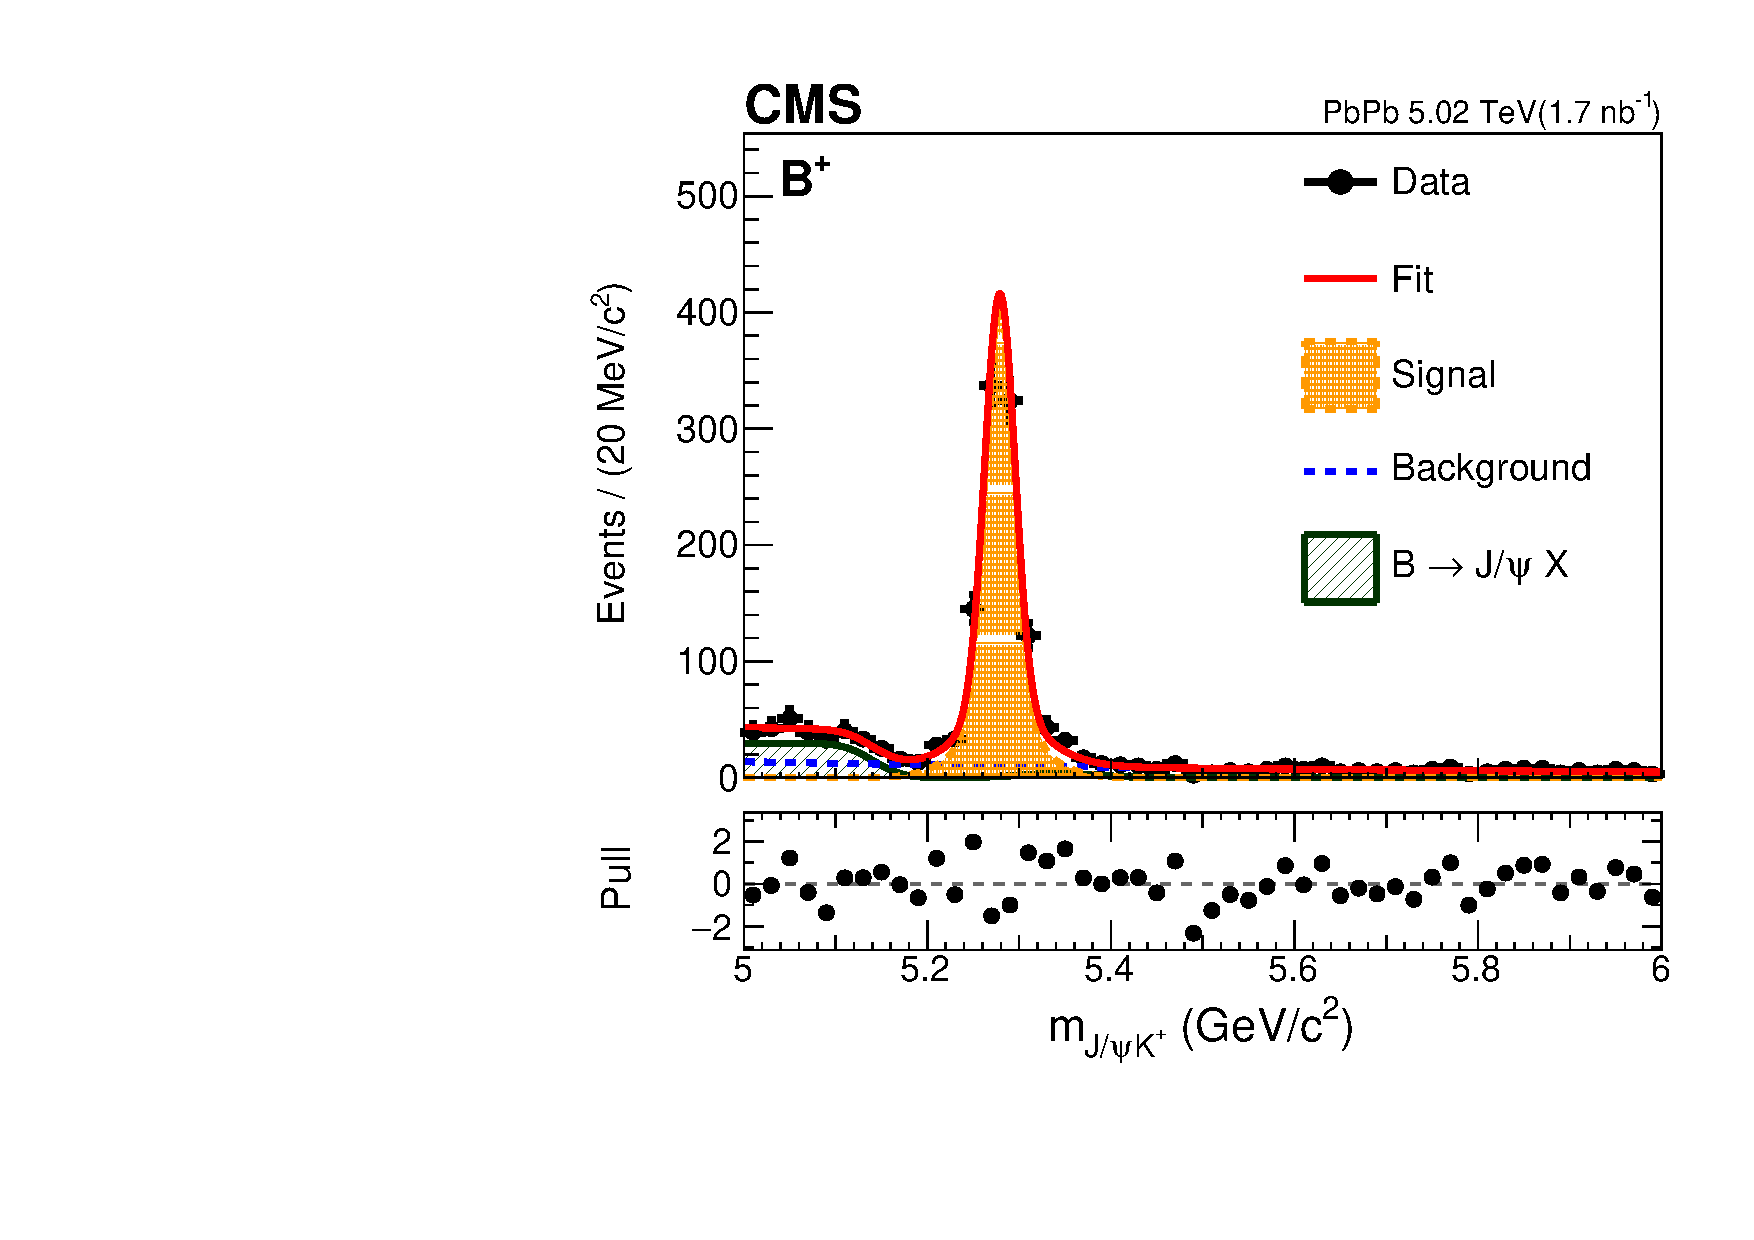
\includegraphics[width=.49\textwidth]{mass_bu.pdf}
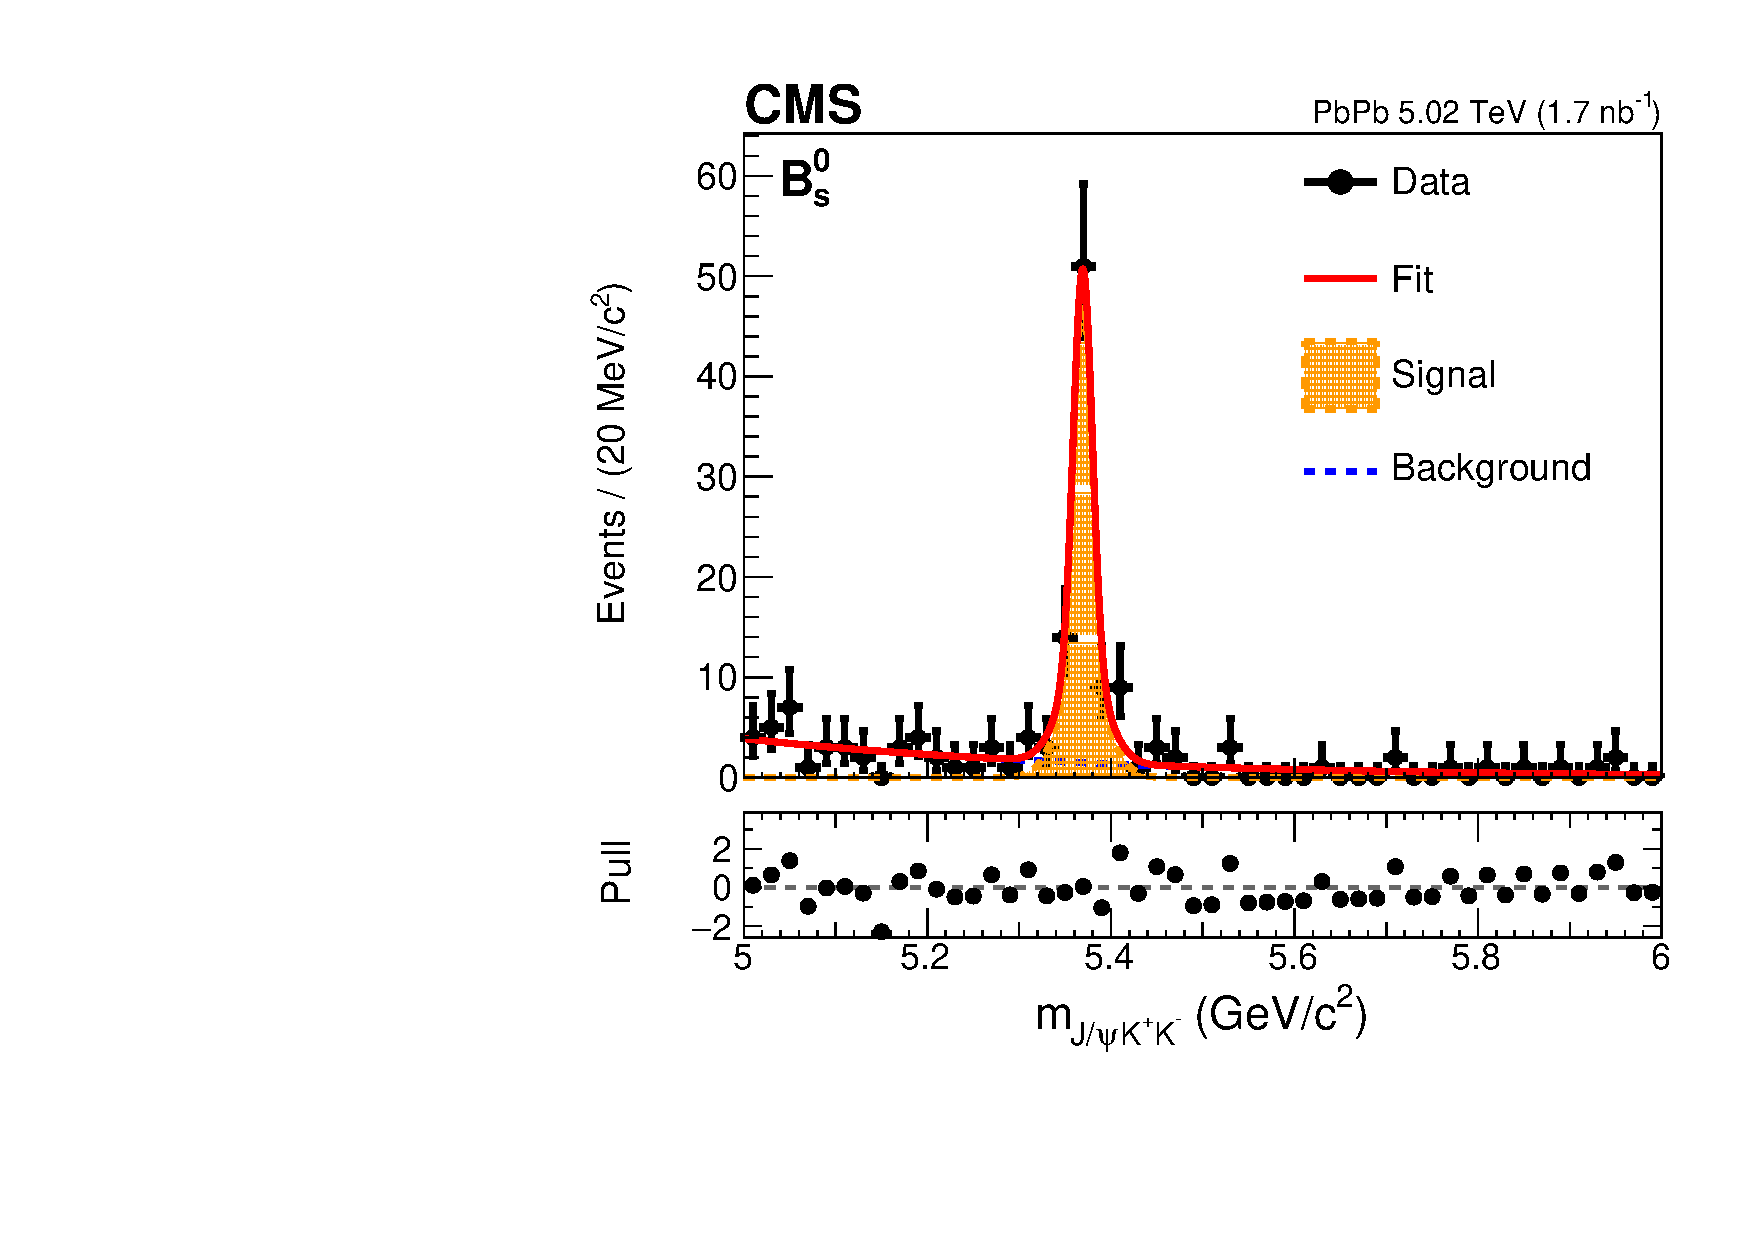
\includegraphics[width=.49\textwidth]{mass_bs.pdf}
\caption{Invariant mass distributions of $\PBp$ (left) and $\PBzs$ (right) candidates, 
%measured in the fiducial regions specified in Eq.~\ref{eq:fid}, 
for event centrality in the range 0--90\%. The lower panels show the pulls, obtained as the difference between the data points and the fit result, divided by the uncertainty in data.}
\label{fig:massPeaks}
\end{figure}
%$range $\abs{y}<2.4$, \pt interval 5--50\GeVc,

The raw \PB\ meson signal yields are extracted using an extended unbinned maximum likelihood fit to the invariant mass spectra. %in the range 5--6$\GeVcc$.
%The estimation of the statistical uncertainties of the fitted raw yields is based on the second derivatives of the negative log-likelihood function.
%
The signal shape is modeled by a sum of two Gaussian functions, with parameters determined from MC simulation, except for the common mean and the overall signal yield that are free parameters of the fit.
%with a common mean (which is a free parameter together with the amplitude), and widths individually determined from MC simulation. 
%The relative contribution of the two Gaussian functions to the signal yield is also fixed at the value given by the MC samples.
The combinatorial background, from uncorrelated combinations of \PJGy\ candidates with extra particles,
gives rise to a falling contribution in the invariant mass spectrum which is modeled by an exponential function.
%a 3rd- (1st-) order polynomial for the case of \PBzs (\PBp). %, as determined from studies of the inclusive $\PJGy$ MC sample.
An additional background source can arise from possible contamination from other b hadron decays.
For the \PBp\ spectrum, partially reconstructed $\PB$ decays, such as ${\text{B}}^{0} \to \PJGy~\PKst^0 \to \mu^{+}\mu^{-}\PKp\Pgpm$, lead to a heightened background in the invariant mass region below 5.2\GeVcc.
The decay $\PBp \rightarrow \PJGy \pi^{+}$, where the pion is misidentified as a kaon, results in a small peaking structure under the signal peak.
Such partially and misreconstructed \PB\ hadron components are modeled from simulation, via an error function and a Gaussian function, respectively; both shapes and the normalization of the Gaussian function (relative to the signal) are fixed in the fit to the data.   
For the \PBzs\ meson case, such background contributions are found to be negligible, as a consequence of the tight selection on the mass of the $\Pphi$ candidate.
%
%As an example, a heightened structure can be created by  decays in which one decay product is lost, resulting in a $\PBp$ (\PBm) candidate.
%
%Examples of
The results of the fits to the invariant mass distributions are shown in Fig.~\ref{fig:massPeaks}.
% for the \pt\ region 15--50\GeVc.

%\comment{enter significance}
The statistical significance of the \PB\ meson signals is estimated from the ratio of likelihoods obtained by fitting the data with the full model and the background-only model. Estimates obtained by this means well exceed 10 standard deviations for both mesons.  
This is the first observation of the \PBzs\ signal in heavy-ion collisions. 

\section{Production yields}

For each \PB\ meson, the production yield is computed in each \pt\ interval according to
%
\begin{equation}
 \frac{1}{\TAA} \frac{{\rd}N}{{\rd}\pt} =  \frac{1}{2 \, \mathcal{B} \, N_{\text{MB}} \, \TAA}
 \frac{N_{\rm{obs}}(\pt)}{\Delta\pt} 
 \times
\left< \frac{1}{\alpha(\pt, y) \times \epsilon(\pt, y)} \right> \, ,
%\left< \frac{1}{\epsilon(\pt, y)} \right> \, ,
% \frac{N_{\rm{obs}}(\pt)}{\alpha(\pt) \, \epsilon(\pt)} \, ,
%\frac{1}{\TAA}\frac{{\rd}N^{\PBzs}_\PbPb}{{\rd}\pt}\right|_{\abs{y}<2.4} = \frac{1}{2} \frac{1}{\mathcal{B} \, N_{\text{MB}} \, \TAA} \frac{1}{\Delta\pt} \left.\frac{N^{(\PBzs+\PABzs)}_\PbPb(\pt)}{\alpha_\PbPb(\pt) \, \epsilon_\PbPb(\pt)}\right|_{\abs{y}<2.4} .
 \label{eq:xsection}
\end{equation}
%
where $N_{\rm{obs}}$ denotes the raw signal yield, extracted in each \pt interval of width $\Delta \pt$.
%
The factor 1/2 accounts for the fact that the raw yield is measured for particles and antiparticles added together while the production yield is given for one species only, and $\mathcal{B}$ stands for the branching fraction of the corresponding decay chain.
%
%For the \pp cross section, $\mathcal{L}$ represents the integrated luminosity, and for the \PbPb cross section,
\NMB\ is the number of minimum bias events and \TAA is the nuclear overlap function~\cite{glauber2007}. 
The \TAA\ is equal to the number of nucleon-nucleon (NN) binary collisions divided by the NN total inelastic cross section, and it can be interpreted as the NN-equivalent integrated luminosity per heavy ion collision. The \TAA value for inclusive \PbPb collisions at $\sqrtsNN=5.02$\TeV is $(5.6\pm0.2)$\mbinv as estimated from an MC Glauber model~\cite{glauber2007}, implemented in the {\sc{tglaubermc}} v3.2 software package~\cite{glauber2017}.
The measurement is performed in a similar fashion as a function of the \PbPb\ collision centrality. The centrality class is represented as the average number of participating nucleons, \npart; the latter, determined using the above Glauber model, is highly correlated with the impact parameter of the collision.
%The above is also employed to obtain the average number of participating nucleons,\npart. This latter number is highly correlated with the impact parameter of the collision, and is used as the abscissa when plotting results as a function of \PbPb collision centrality.

The acceptance and the efficiency factors, the last term in Eq. (\ref{eq:xsection}), are obtained employing 2D fine-grained maps of the acceptance $\alpha (\pt,y)$ and the efficiency $\epsilon(\pt,y)$.
These maps are determined from MC simulation samples of \PB\ meson signal events, generated within the analysis fiducial region given by: $\abs{y}<1.5, \; \pt>10\GeVc; 1.5<\abs{y}<2.4, \; 7<\pt<50\GeVc$.
%
The acceptance corresponds to the fraction of generated events passing the muon and kaon selection thresholds specified in Section~\ref{sec:sel}, while the efficiency is determined as the fraction of accepted events that pass the full analysis selection criteria, including the trigger.
%
The maps are used to determine the $1/(\alpha\times\epsilon)$ value for each \PB\ candidate in data, based on the kinematics $(\pt,y)$ of the candidates, and the corresponding average $\langle 1/(\alpha\times \epsilon)\rangle$ obtained for the candidates within a 160\MeVcc window centered on the \PB\ meson's world-average mass. 
%and averaged over the signal region of the data sample. 
The MC-derived efficiency maps are corrected by data/MC scale factors for the muon reconstruction and trigger efficiencies, which are obtained applying the ``tag-and-probe" method using the \PJGy\ resonance~\cite{Khachatryan:2010zg}.
%\comment{tag and probe}
%


\section{Systematic uncertainties}

The cross section measurements are affected by several sources of systematic uncertainties arising from the signal extraction, acceptance and efficiency, $\mathcal{B}$, \NMB, and \TAA\ determinations.

The uncertainty from the signal and background modeling is evaluated by considering the following fit variations:
(i) using low-order polynomials for describing the combinatorial background, 
(ii) using a sum of three Gaussian functions with a common mean for alternatively describing the signal,
(iii) varying the widths of the signal double-Gaussian function by 10\% (to account for possible mismatches in mass resolution between simulation and data), and
(iv) fixing the common Gaussian mean to its MC simulation value. 
%(iii) fixing the mean of the Gaussian function to the value determined from simulation;
%(iv) releasing the MC-based constraint on the width of the signal double Gaussian, by allowing a common resolution scale factor to float in the fit.
%(i) increasing/decreasing the width parameters determined from simulation by XXX\% (the maximum relative statistical uncertainty of the fitted width parameter among all \pt bins); (ii) using a single Gaussian function; (iii) using a sum of three Gaussian functions with a common mean, and (iv) fixing the mean of the Gaussian function to the value determined from simulation. %CHECK this!
%The uncertainty in the modeling of the combinatorial background is similarly evaluated by varying the corresponding probability distribution functions to a lower-order polynomial and exponential function.
The maximum of the signal variations and the maximum of the background variations are added in quadrature as the systematic uncertainty from fit modeling. The range of the modeling uncertainties is 1.2 - 6.4\% for \PBzs\ and 2.5 - 4.5\% for \PB\

%The systematic uncertainty due to the selection of the $\PB$~meson candidates is estimated by varying the selection applied to the BDT variable, for data and MC samples, dividing the resulting yields and taking the difference with respect to unity. The maximum difference obtained for the scanned values is propagated as the systematic uncertainty. \comment{check statcomm guidelines}
%comparing the BDT-obtained nominal result with the results using a cut-based method (a rectangular cut) that uses the Genetic Algorithm to determine the best cut value for each parameter~\cite{Hocker:2007ht}.The same signal and background shape parametrization are used, and the same analysis parameters are optimized as in the BDT nominal method. The significance is similar for the two methods ($\sim$8). This provides an estimate of the potential difference between different selection criteria. The full difference between the two methods is propagated as a systematic uncertainty.
%For the \PbPb results, because of the small signal in data, in order to minimize the impact of statistical fluctuations, a different approach was taken. In this case, the $\PBzs$ selection uncertainty was estimated using the pp data sample, as the full difference in the yield between the \Pp\Pp\ results with the BDT trained on the \Pp\Pp\ sample (the nominal result) and the results with the BDT trained on the \PbPb sample (the selection used for the \PbPb results).

%The bin-by-bin systematic uncertainties associated with the acceptance correction are estimated by varying the shape of the generated $\PB$~meson \pt and $y$ spectra. For the purpose of the systematic studies only, both data and MC are split into four \pt and $y$ bins. The ratio between data and simulated \pt spectra (including their statistical uncertainties) is used to generate pseudo-experiments (`toys'). Each toy is fit with a polynomial, which is then used to reweight the MC $\PB$~meson \pt spectra. A new acceptance value is calculated for each modified shape, for each kinematic bin. The root mean square (RMS) of all acceptances determined via toys is propagated as the systematic uncertainty by choosing the maximum RMS value emerging from the \pt and $y$ shape variations.
%\comment{update remaining of para}
%Because of the small signal available, for the \PbPb results the \Pp\Pp\ ratio is used to generate the toys. 

The systematic uncertainties associated with the limited size of the MC simulation samples are obtained by re-computing the 2D fine-grained $\alpha(\pt,y) \times \epsilon(\pt,y)$ maps and the corresponding $\langle 1 / (\alpha\!\times\!\epsilon)\rangle$ averages over the data sample.
The statistical uncertainties from the MC-derived acceptance$\times$efficiency
%$\alpha\!\times\!\epsilon$ 2D maps
are propagated by generating 10000 2D maps (per bin in the differential measurement), where each entry is obtained by randomly sampling 
the $\alpha\!\times\!\epsilon$ values from Gaussian distributions with widths given by the statistical uncertainty. The resulting systematic
uncertainties are obtained as the width of the $\langle 1 /(\alpha\!\times\!\epsilon\rangle)$ distribution from the alternative 2D maps. 
%Most of the systematic uncertainties come from selection efficiency $\frac{1}{\epsilon}$. %divided by its central value
The range of the MC event count uncertainties is 2.4 - 27.6\% for \PBzs\ and 1.9 - 9.2\% for \PB\


\begin{table}[h]
\begin{center}
\topcaption{Summary of systematic uncertainties in the production cross section measurements for \PBp\ and \PBzs\ mesons
for centrality ranges 0-30\%, 30--90\%, and 0--90\%. 
The measurements are performed in the \PB\ meson kinematic region given by $10<\pt<50\GeVc$ and $|y|<2.4$. 
%within the analysis fiducial region specified in Eq.~\ref{eq:fid}, 
The relative uncertainty values are shown, in percentage.
%\comment{Acceptance variation has been dropped as systematics (what would it be anyway?!); MISSING: B+: recompute ``total''; Bs: fill in table. ALTERNATIVE: instead of the 3 centrality bins could use the 4 \pt bins employed in the ratio (could even include both, as arc may have different preferences)}
}
\vspace{1em}
\label{tab:syst}
  \begin{tabular}{ l  {c}@{\hspace*{5pt}} ccc {c}@{\hspace*{5pt}}  ccc  }
%    \hline
                                    && \multicolumn{3} {c} {\PBp}   && \multicolumn{3} {c} {\PBzs} \\
    \cline{1-1}\cline{3-5}\cline{7-9}
    Centrality class           && 0--30\% & 30--90\% & 0--90\%  && 0--30\% & 30--90\% & 0--90\% \\ 
    %\vspace{1cm}
 %   \cline{1-1}\cline{3-5}\cline{7-9}
\multirow{2}{*}{Muon efficiency}\rule{0pt}{3ex}
			              && $+$3.2  & $+$3.1   & $+$3.1     && $+$3.8   & $+$3.2  & $+$3.6 \\
                                      && $-$3.0  & $-$2.9   & $-$2.9     && $-$3.5   & $-$3.0  & $-$3.3 \\
    Data/MC agreement                 && 13    & 8.0     & 11       && 2.6    & 3.2   & 2.7  \\
    MC sample size                    && 3.3   & 2.3     & 2.5      && 7.2    & 2.4   & 4.7  \\
    PDF variation                     && 2.5   & 2.8     & 2.6      && 2.5    & 3.2   & 2.3  \\
    Tracking efficiency               && 5.0   & 5.0     & 5.0      && 10     & 10    & 10   \\
    \TAA                              && 2.0   & 3.6     & 2.2      && 2.00   & 3.6   & 2.2  \\
%  \multirow{2}{*}{\NMB (event selection)} 
%  				      && +1.3  & +1.2  & +1.2   && +1.3  & +1.2  & +1.2 \\
%                                     && -1.3  & -1.2  & -1.2   && -1.4  & -1.2 &  -1.2 \\
\NMB (event selection)                &&  1.3  &  1.2  &  1.2   &&  1.4  &  1.2 &   1.2 \\
%   \hline                                         
%    Total                           && +12.7  & +13.3  & +13.1    && +16.6  & +13.5  & +14.4 \\
%                                    && -12.4   & -13.0   & -12.9    && -15.9  & -13.2  & -13.8 \\
%    \hline
%    \pt shape                         && 0.13  & 0.16    & 0.14     && 0.03   & 0.01  & 0.01 \\
%    Closure test                      && 0.57  & 0.20    & 0.28     && 1.21   & 3.03  & 1.09 \\
%    sPlot Weight                         && 0.22    & 0.38     & 0.24       && 0.47    & 1.58   & 0.59  \\
    \vspace{-2mm} \\
%    \cline{3-5}\cline{7-9}
    Branching fraction && \multicolumn{3} {c} {2.8\;\,} && \multicolumn{3} {c} {7.6\;\,} \\
    \hline
\end{tabular}
\end{center}
\end{table}



The efficiency and acceptance determinations, based on MC simulation, are further affected by potential disagreements between data and MC .
The signal MC simulation is validated against data by inspecting the distributions of the variables employed in the selection. The signal distributions are extracted from the data employing the sPlot method~\cite{splot}, using the mass of the B-meson candidates as discriminating variable, and are also cross-checked with a simple %the alternative 
sideband-subtraction method. In particular, the sPlot-derived signal distributions for the BDT score are retrieved from the data, along with the corresponding data/MC ratios. These ratios are in turn used to re-weight the MC simulation, and the resulting deviation in the $\langle 1 / (\alpha\!\times\!\epsilon)\rangle$ factors are assigned as systematic uncertainties. %from this source.
%
This procedure is employed using the higher-yield channel, namely the \PBp.
For the \PBzs\ meson, the limited size of the data sample yields results that are compatible between data and simulation, within the statistical uncertainties. As such, the \PBp\ channel is used as the calibration mode for the \PBzs\ channel. %given the similar decay topologies. 
A procedure identical to that described above, applied to the \PBp\ sample, is employed but using only tracking related variables.
The systematic uncertainty for the \PBzs\ corresponds to that evaluated for the \PBp\ and further taking the maximum of the deviation determined from tracking related variables to account for the presence of an extra track in the \PBzs\ channel..

%The data/MC efficiency differences have been further estimated using data-driven efficiency measurement methods.
%Data-driven efficiency measurement methods are employed to further estimate data/MC efficiency differences have been further estimated using 
The uncertainty in the efficiency of the muon trigger, reconstruction, and identification is evaluated using a tag-and-probe technique using the \PJGy\ meson in data~\cite{Khachatryan:2010zg}. The derived data/MC scale factors are employed in the determination of the nominal $\alpha\!\times\!\epsilon$ 2D maps, while the associated uncertainties are propagated as systematic uncertainty in the  $\langle 1 / (\alpha\!\times\!\epsilon)\rangle$ factors.
The difference in the track reconstruction efficiency in data and simulation was estimated by comparing 3-prong and 5-prong \PDst decays, \dstardecay~\cite{Khachatryan:2016odn}. 
%A relative systematic uncertainty of 5\% per hadron track is also considered~\cite{Khachatryan:2016odn}, to account for the uncertainty in the track reconstruction efficiency.
%This uncertainty propagates to
 This results in 5\%  (10\%) uncertainty in the efficiency determination for the \PBp\  (\PBzs) decay for involving one (two) kaon(s).

The determination of the $\langle 1 / (\alpha\!\times\!\epsilon)\rangle$ factors, for each analysis bin, involves averaging over the data. In order to reflect this statistical effect, the overall statistical uncertainty from the \PbPb\ data is calculated using a bootstrap method~\cite{bootstrap}, where data events are resampled 1000 times with replacement. The corrected yield is re-determined for each bootstrap sample, and the spread of its distribution is assigned as the statistical uncertainty.   


Various consistency checks of the analysis procedure have been performed, which do not result in additional systematic uncertainties.
%
The consistency of the fitting procedure was verified by generating and fitting pseudo-experiments using the likelihood model and parameters employed for fitting the data. Pull distributions show random behavior consistent with unit Gaussians.
%
%The fitting procedure has been validated using the MC samples, as well as pseudo-experiments (\ie mass spectra generated from the fitting model itself). 
A consistency check %, so-called closure test, 
was performed using MC simulation, where the signal yields are extracted with the fitting procedure and the acceptance and efficiency corrections applied, thus retrieving the generated yields. %The closure of this test is within 3\%. 
%
Potential biases in the acceptance and efficiency calculations associated with the shape of the \PB\ mesons kinematic distributions from simulation were probed by re-weighting the  {\PYTHIA} simulation according to varied \pt\ shapes %such as linear, quadratic, linear + inverse, linear + square root, and linear + logarithmic function,
 and recomputing the factors $\langle 1 / (\alpha\!\times\!\epsilon)\rangle$. Such deviations were found to be negligible. 
This confirmed independence from the MC is expected in view of the fine-grained 2D $\alpha\!\times\!\epsilon$ MC maps and the $\langle 1 / (\alpha\!\times\!\epsilon)\rangle$ averaging based on data, and further attests to the robustness of the analysis procedure. 
The effect of background contamination % within the signal region, 
in the averaging procedure was studied employing the sPlot method and was found to be negligible.  

%The uncertainty for \NMB accounts is due to the inefficiency of the event selection and the trigger in selecting hadronic events~\cite{Khachatryan:2016odn}.
%
The systematic uncertainties in the Glauber model normalization factor (\TAA) are derived from propagating the uncertainties in the event selection efficiency, and in the nuclear radius, skin depth, and minimum distance between nucleons in the Pb nucleus parameters of the Glauber model~\cite{Khachatryan:2016odn}. The uncertainties associated with the branching fraction of the decay chains $\mathcal{B}$ are obtained from Ref.~\cite{pdg2018}.
%
The $\mathcal{B}$ factor is common to all bins in the cross section measurements, as is the case also of \TAA\ and \NMB\ in the \pt-differential results; the corresponding uncertainties are denoted global uncertainties.  
%The values of $\mathcal{B}$ do not vary bin-to-bin in the cross section measurements, as is the case also of \TAA\ and \NMB in the \pt-differential results, and the corresponding uncertainties are denoted global uncertainties.  
%
%The uncertainties in \TAA, \NMB, $\mathcal{B}$ ($\mathcal{B}$) do not vary bin-to-bin and are denoted global uncertainties in the \pt (centrality) differential cross section measurements.  
%These are global uncertainties in the cross section measurements.  
%
The total systematic uncertainties in the cross section measurement are computed as the sum in quadrature of the different contributions mentioned above, which are summarized in Table~\ref{tab:syst}. 


\begin{figure}[t]
\centering
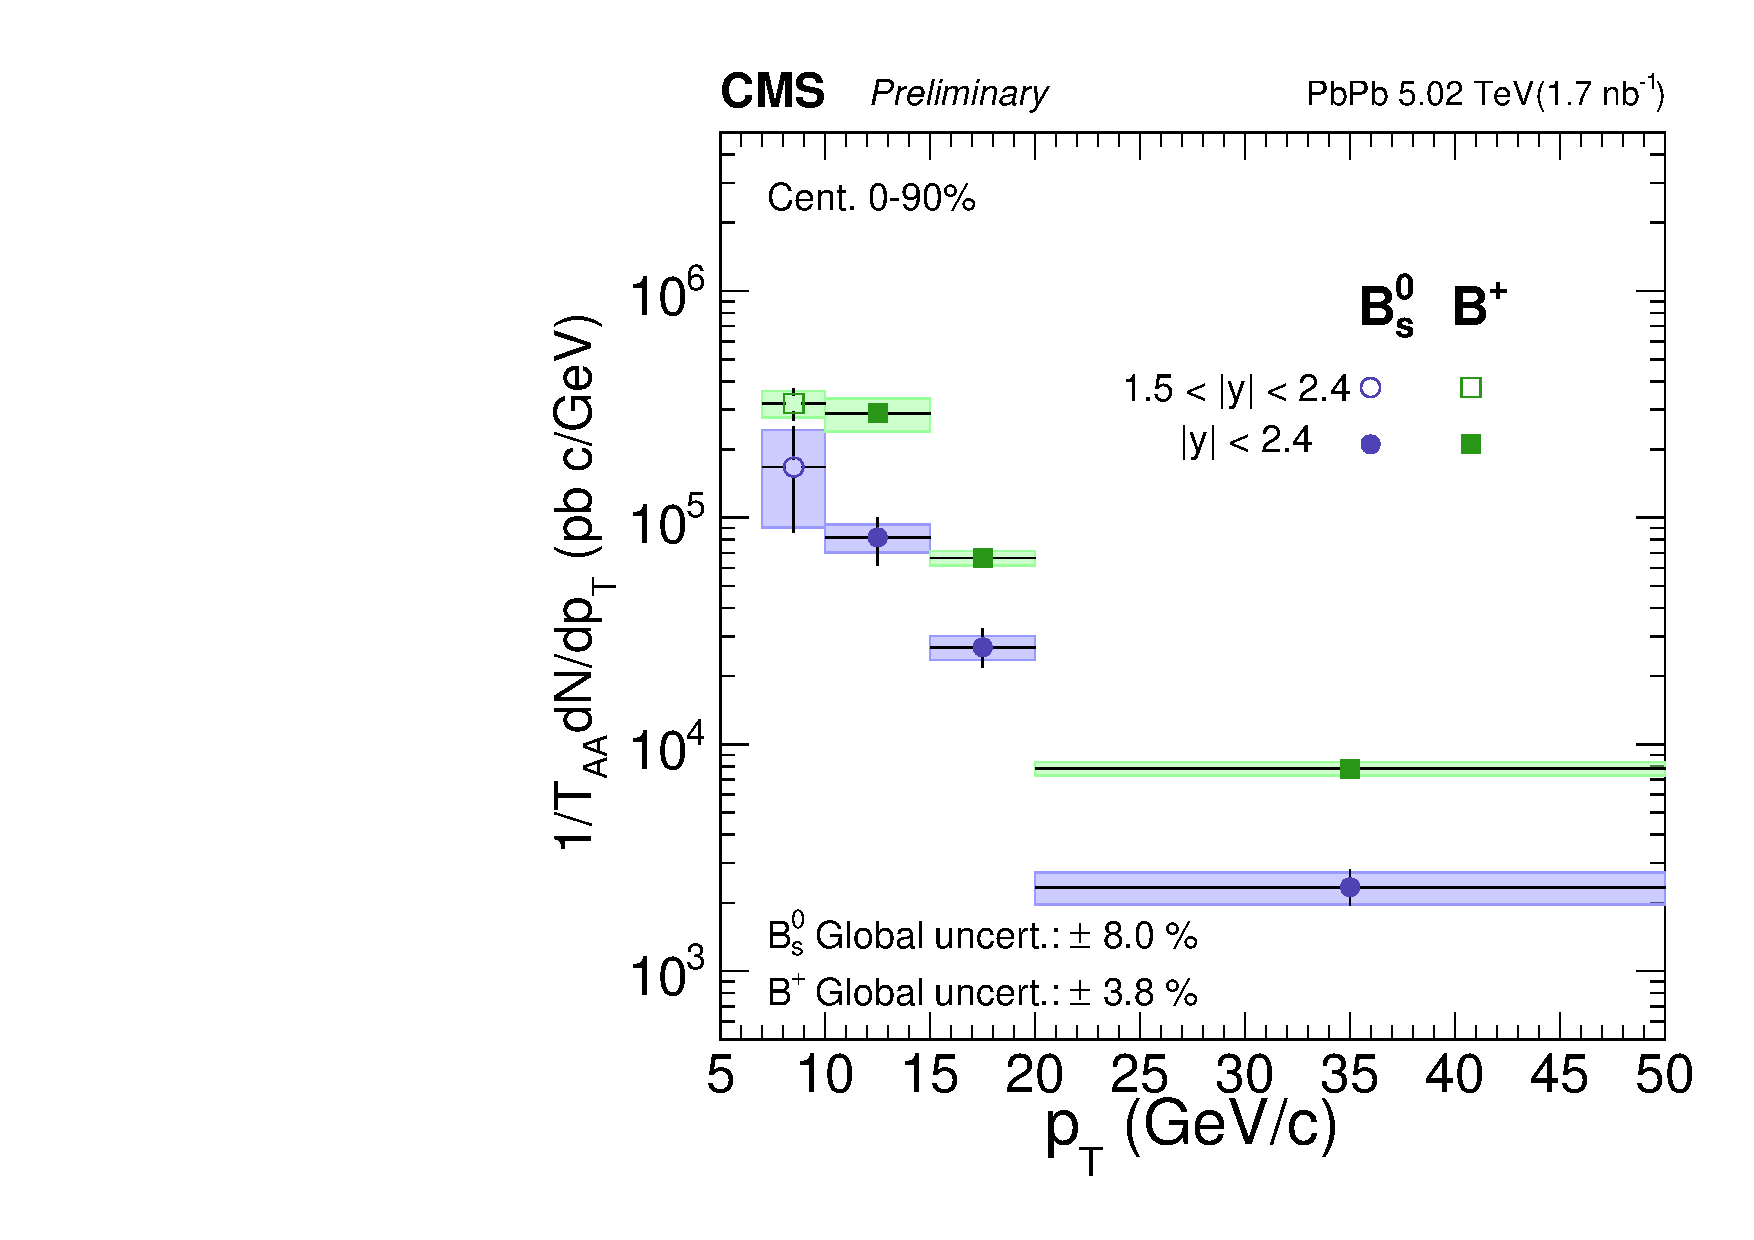
\includegraphics[width=.48\textwidth]{xsect_vsPt.pdf}
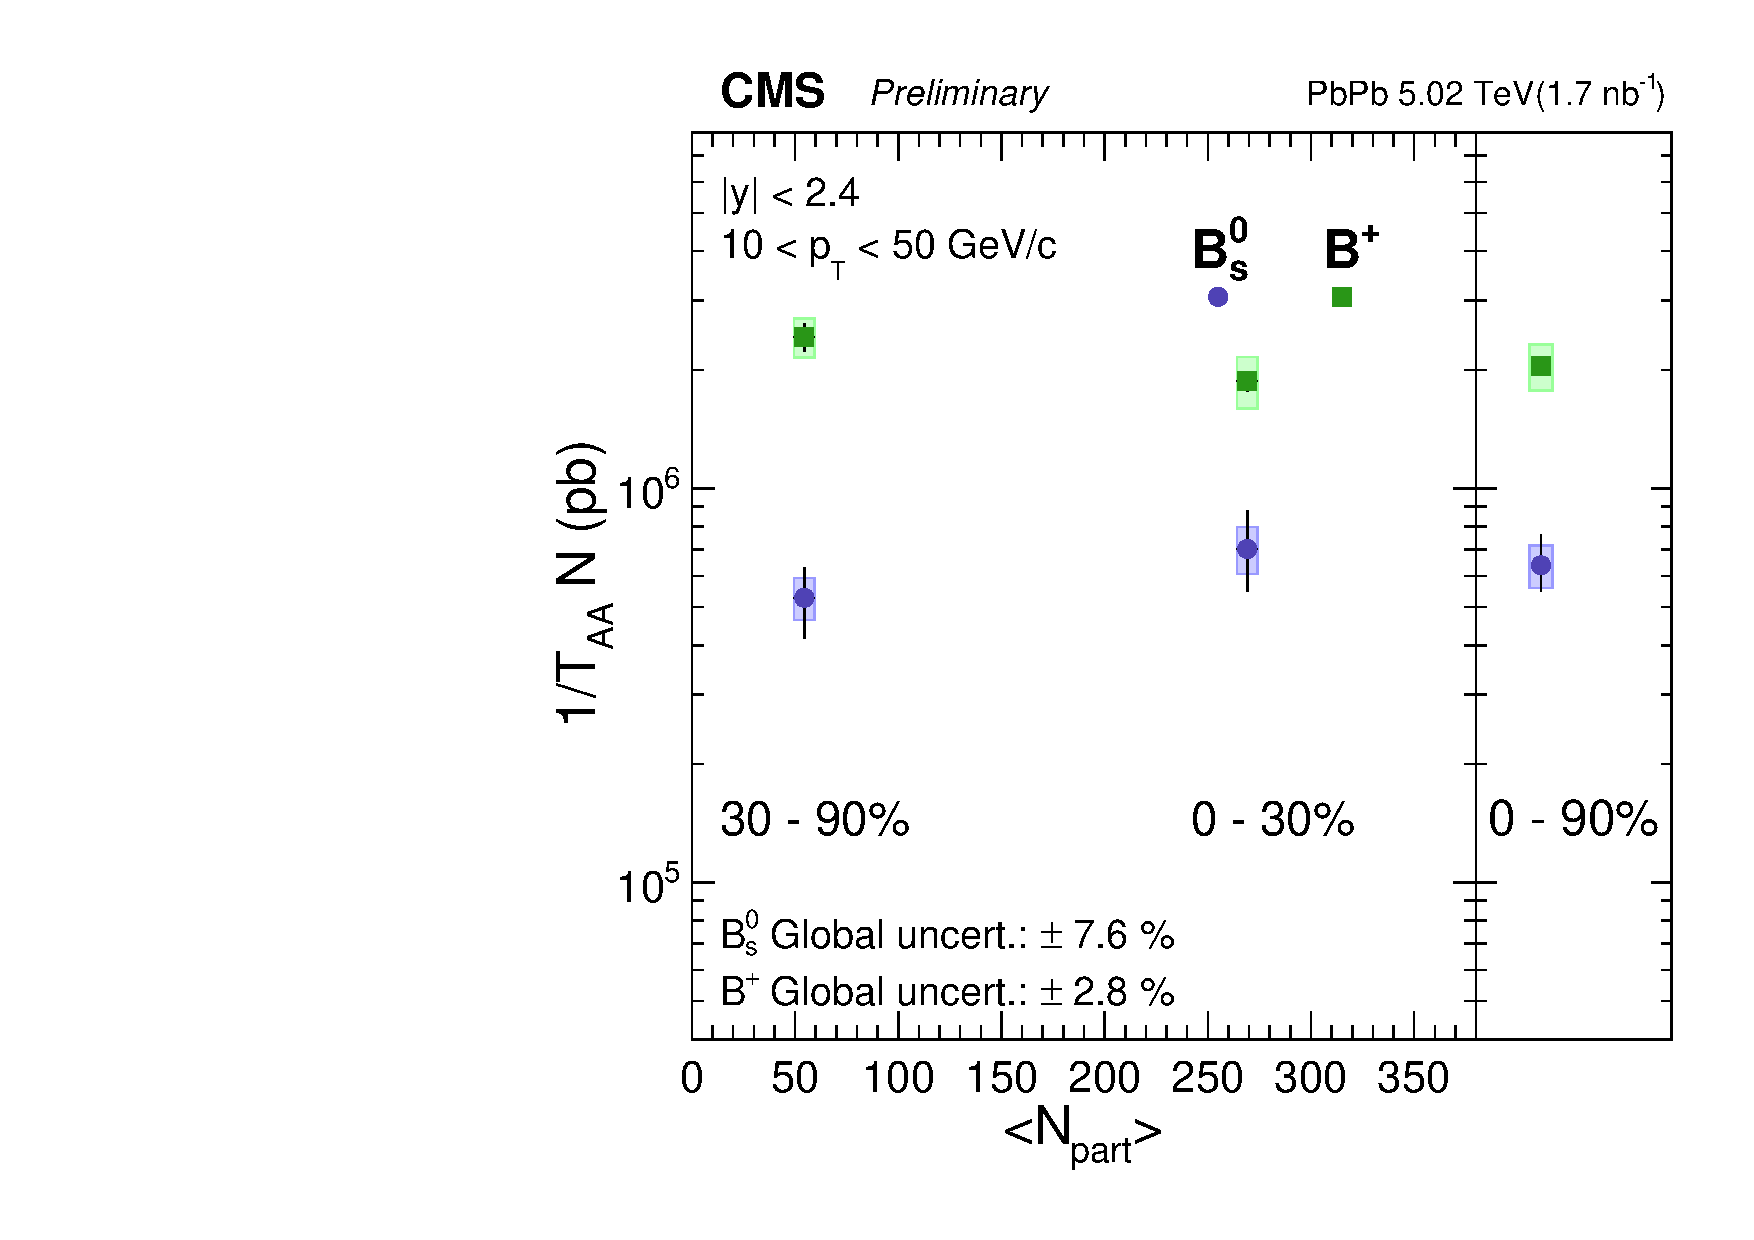
\includegraphics[width=.48\textwidth]{xsect_vsCent.pdf}
\caption{The acceptance- and efficiency-corrected yields for the \PBp\  and \PBzs\ mesons, scaled by \TAA and \NMB\ in \PbPb\ collisions at $\sqrtsNN=5.02\TeV$. The results are shown as a function of the meson \pt (\cmsLeft), and of the event centrality (\cmsRight), where the rightmost panel indicates the centrality-integrated result.  The vertical bars (boxes) correspond to statistical (systematic) uncertainties. The global systematic uncertainty comprises the uncertainties in \TAA, \NMB, $\mathcal{B}$ (\cmsLeft) and $\mathcal{B}$ (\cmsRight).
}
\label{fig:xsections}
\end{figure}
%%%%%The measurements are performed in the analysis fiducial region of Eq.~\ref{eq:fid}.  
%in two \pt intervals from 7 to 50\GeVc.



\section{Yield ratio}

The differential production yields for \PBzs\ and \PBp\ mesons in PbPb collisions, Eq.~\ref{eq:xsection}, 
%measured in the analysis fiducial region of Eq.~\ref{eq:fid},
are presented in Fig.~\ref{fig:xsections} as functions of the mesons \pt\ (\cmsLeft) and event centrality (\cmsRight).

The ratio of production yields of the \PBzs\ and \PBp\ mesons
%, measured in the same fiducial region, 
is formed as
%
\begin{equation}
R = \frac{N^{\PBzs}}{N^{\PBp}} = 
\frac{N_{\rm{obs}}^{\PBzs}}{N_{\rm{obs}}^{\PBp}}
\frac{ \mathcal{B}^{\PBp}}{ \mathcal{B}^{\PBzs}} 
\frac{\langle 1/(\alpha^{\PBzs} \times \epsilon^{\PBzs})\rangle}
     {\langle 1/(\alpha^{\PBp}  \times \epsilon^{\PBp} )\rangle}
%\frac{\alpha^{\PBp}}{\alpha^{\PBzs}}
%\frac{\epsilon^{\PBp}}{\epsilon^{\PBzs}}
\, .
\label{eq:ratio}
\end{equation}
%

\begin{figure}[t]
\centering
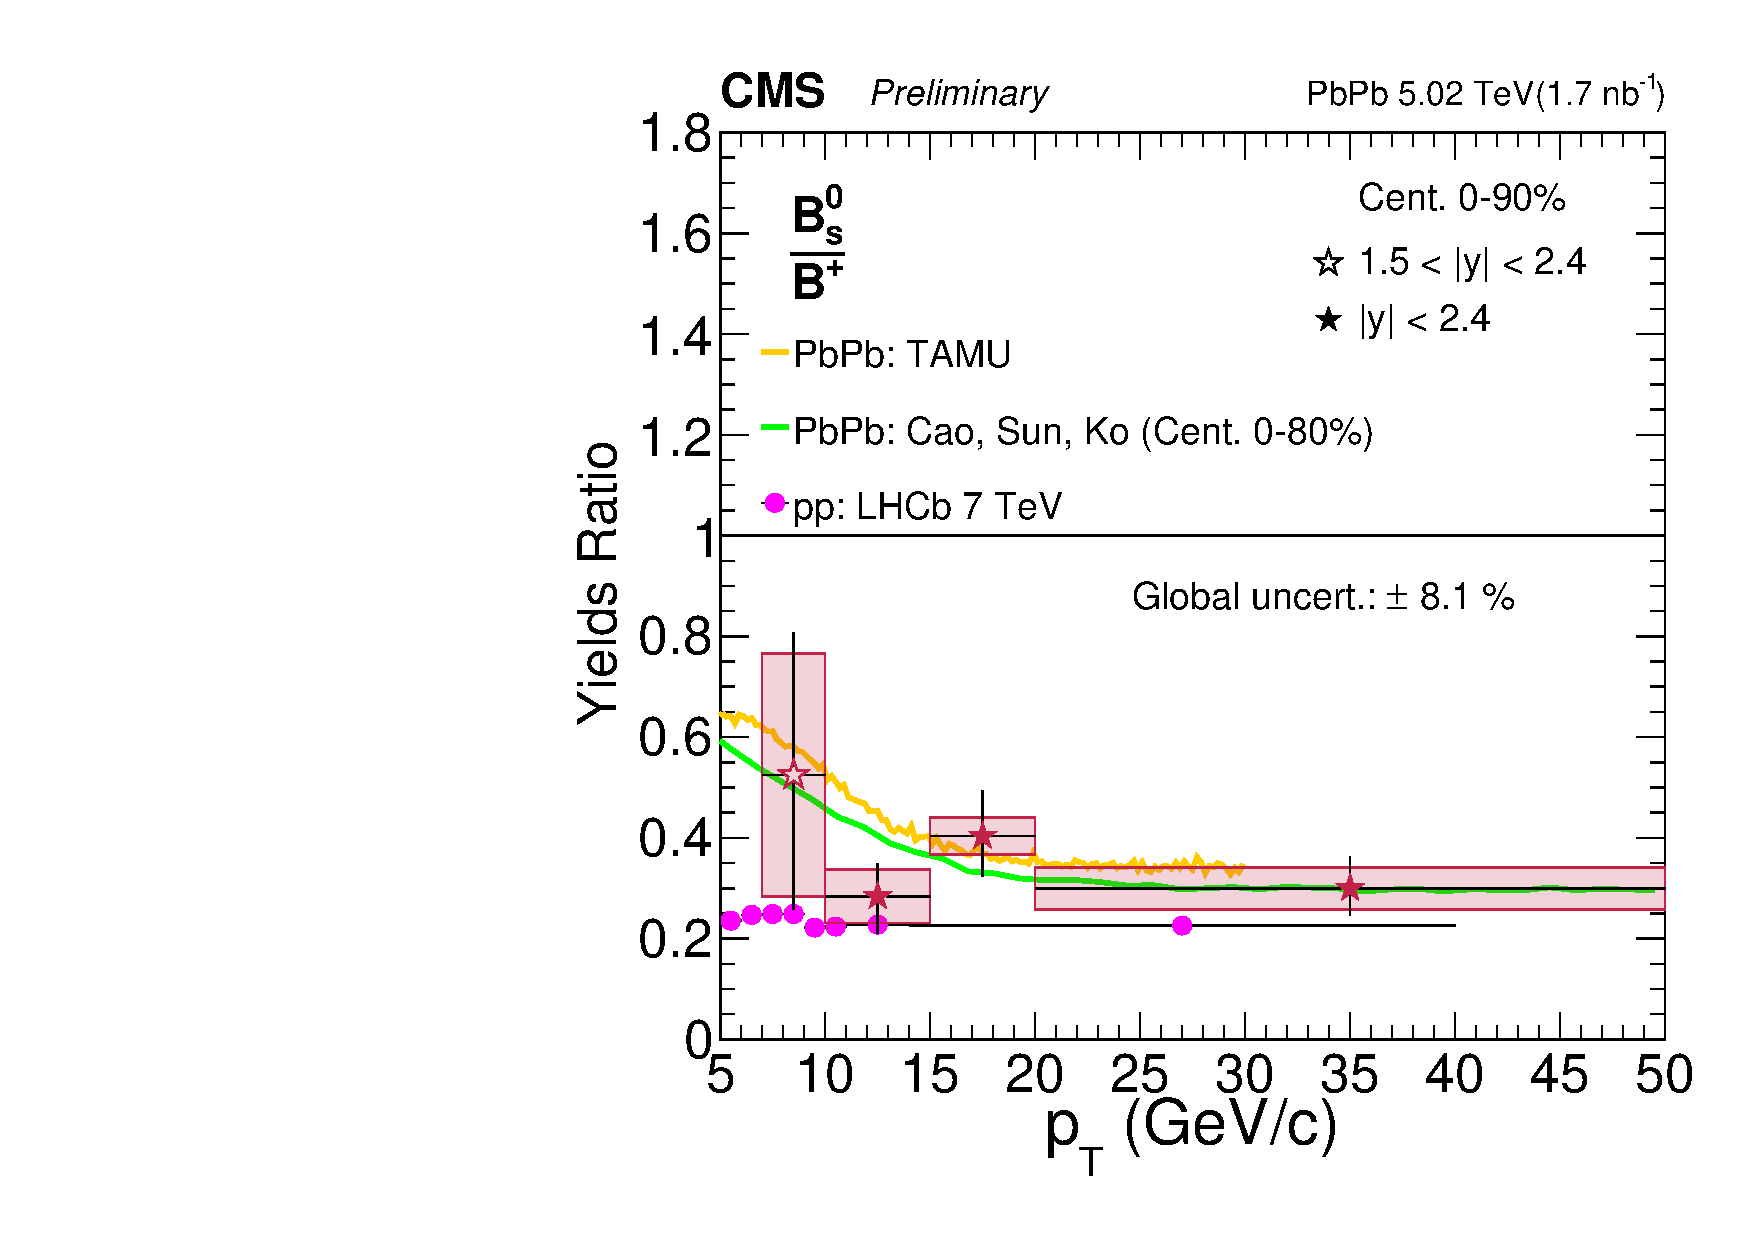
\includegraphics[width=.48\textwidth]{ratio_bsbu_vsPt.pdf}
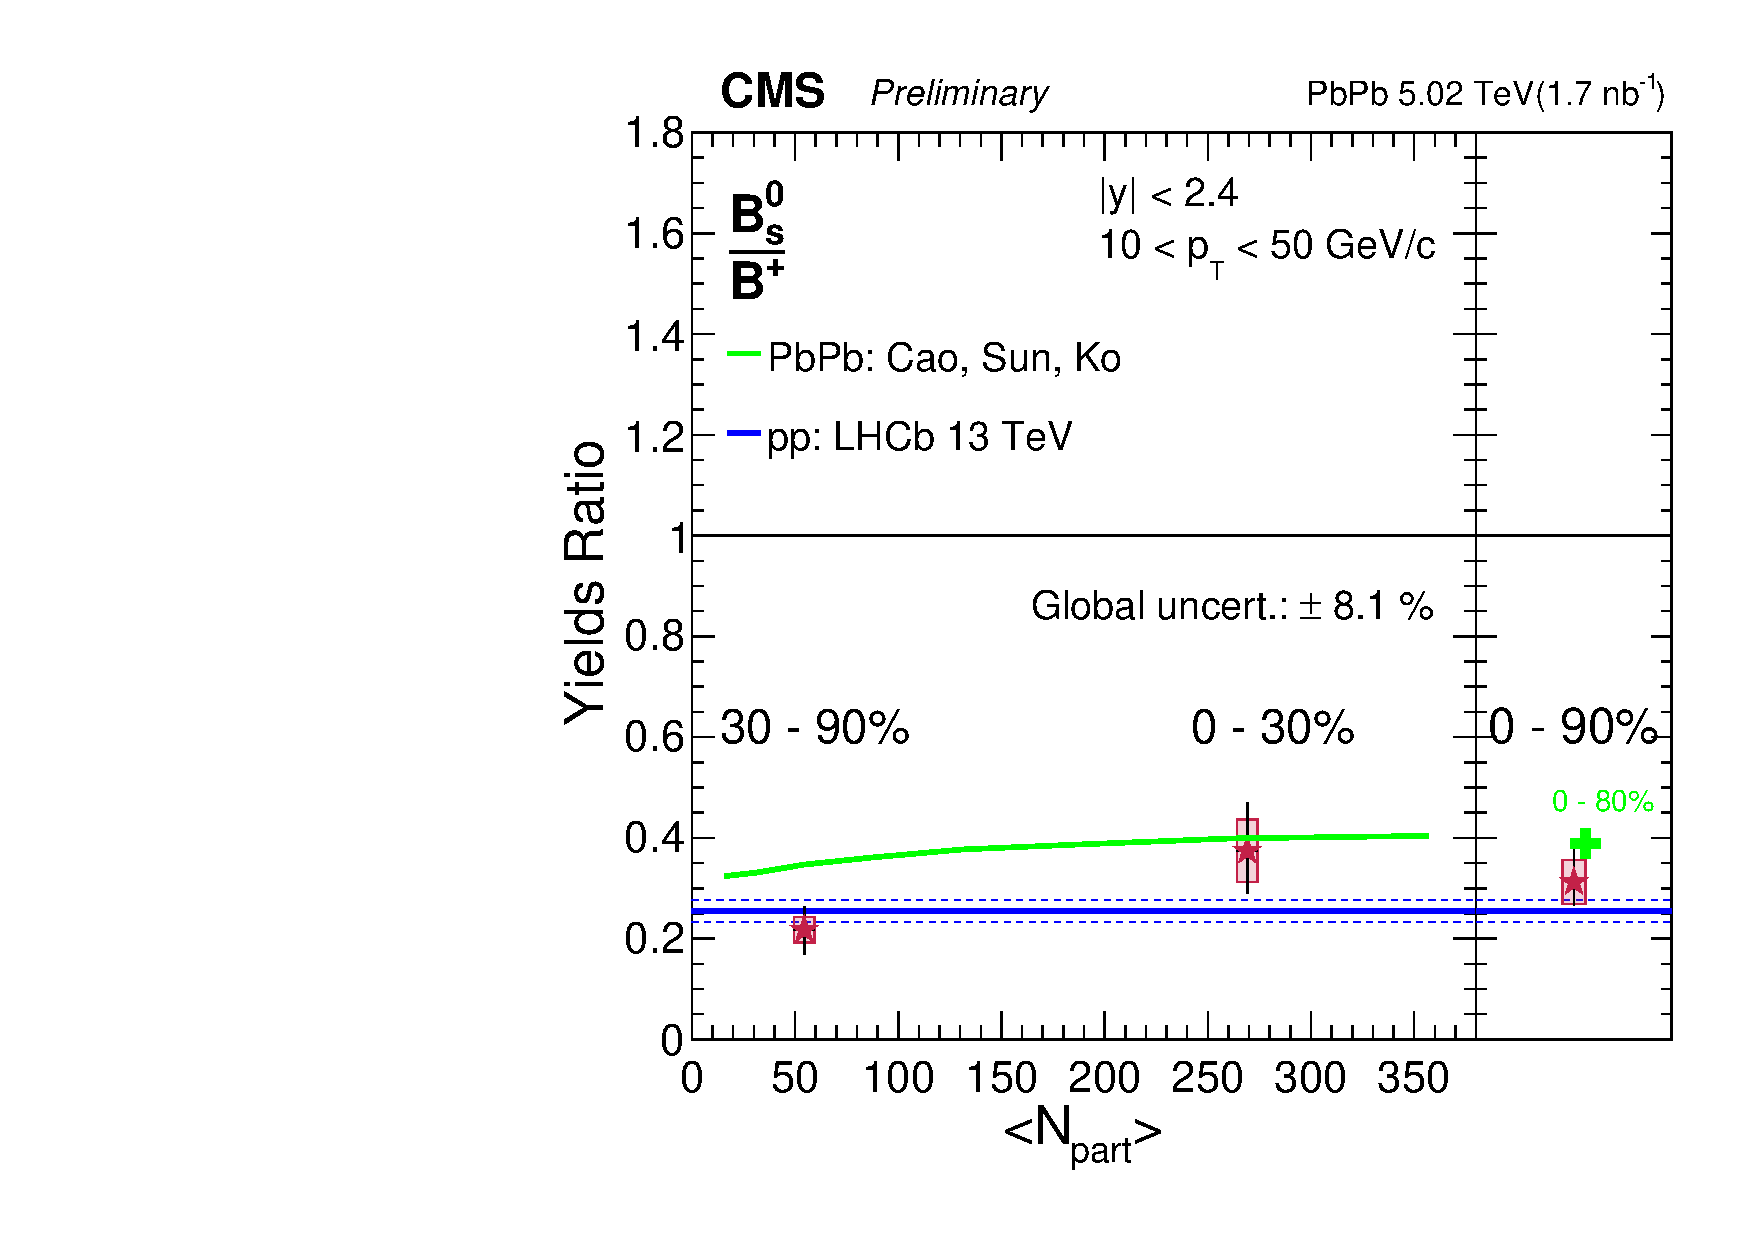
\includegraphics[width=.48\textwidth]{ratio_bsbu_vsCent.pdf}
\caption{The ratio of production yields between \PBzs\ and \PBp\ mesons. 
(\cmsLeft) The ratio dependence on the meson \pt; a prediction from the TAMU transport model~\cite{tamu14}, and the $f_s/f_u$ \pt dependence by LHCb~\cite{fsfulhcb2020} in \pp collisions at 7\TeV are also displayed. 
(\cmsRight) The ratio dependence on the collision centrality; 
the average $f_s/f_u$ result obtained in \pp 7\TeV collisions by LHCb~\cite{fsfulhcb2020} is also displayed as a horizontal bar; 
the rightmost panel shows the centrality-integrated measurement.  
The vertical bars (boxes) correspond to statistical (systematic) uncertainties.
The global systematic uncertainty on the yields ratio corresponds to the decay branching fractions $\mathcal{B}$.}
\label{fig:ratio}
\end{figure}

The terms associated with the size of the data sample (\TAA, \NMB) cancel in the ratio $R$. 
%In the calculation of the systematic uncertainties for the ratio $R$, global-event related uncertainties (\TAA, \NMB) cancel completely. 
Correlated systematic uncertainties associated with the efficiency determination are partially reduced. 
For the tracking efficiency, a 5\% uncertainty is assigned, following from the different number of hadron tracks in the two decays.
Muon efficiency uncertainties from tag-and-probe are determined by varying coherently the efficiency factors in the numerator and denominator within the corresponding uncertainties. 
For the determination of uncertainties related to data/MC comparisons, an identical procedure to that used for the cross sections is employed but using only tracking related variables, using the \PBp\ channel. 
The dominant uncertainty arises from data/MC agreement and a limited MC sample size. 
%\comment{confirm this is the case, and indicate the error ranges}
%
The $R$ ratio results 
%are also determined in the fiducial region specified in Eq.~\ref{eq:fid}, and 
are shown in Fig.~\ref{fig:ratio} 
as functions of the mesons \pt\ (\cmsLeft) and event centrality (\cmsRight).

 The \pt dependence of the ratio $R$ is compared to 
 %the \PBzs\ prediction of a perturbative QCD based model that includes both collisional and radiative energy loss, (CUJET3.0)~\cite{Xu:2015bbz, Xu:2014tda, Xu:2014ica}, and 
 a transport model (TAMU) based on a Langevin equation that includes collisional energy loss and heavy-quark diffusion in the medium~\cite{tamu14}.
 The prediction accounts for recombination contributions to \PBzs meson yield, which are expected to be more significant at low \pt. 
 %reflects the contribution from recombination processes, which are included in the TAMU but not in the CUJET3.0 model. 
% The results measured for $\pt>7$\GeVc have the power to disentangle the two models, albeit after an increase in precision, which can be achieved with a bigger data sample.
%
%Measurements of the \PBzs\ and \PBp\ fragmentation fractions have been performed at the LHC by ATLAS and LHCb~\cite{fsfulhcp2013, Aaij:2013qqa}. 
%An average ratio of the \PBzs\ and \PBp\ fragmentation fractions has been determined by LHCb to be  $f_s/f_u =0.256\pm0.020$~\cite{fsfulhcb2013} in  \pp collisions at 7\TeV. 
%in non-nuclear collisions, including measurements by the LHCb~\cite{Aaij:2013qqa} and ATLAS Collaborations~\cite{Aad:2015cda}.
%
The ratio of the \PBzs\ and \PBp\ fragmentation fractions has been determined by LHCb to be  $f_s/f_u =0.244\pm0.012$~\cite{fsfulhcb2020} in  \pp collisions at 13\TeV, for \PB mesons transverse momenta from 4 to 25\GeVc and pseudorapidity 2 to 5. While no rapidity dependence of the ratio on rapidity has been reported, a decrease with \pt has been observed therein. 
%The same ratio has been more recently measured by LHCb~\cite{fsfsulhcb2019}  at 13\TeV \pp collisions, where a decrease with \pt has been also reported. 
The results are compatible with both the model prediction for \PbPb collisions and the \pp reference results. However, no significant \pt dependence can be established with the precision allowed by the current data. 
%
%The results are compatible with the model, however no significant \pt dependence can be established with the precision allowed by current data. 
%As is displayed in Fig.~\ref{fig:ratio} (\cmsLeft), the data  
%The $R$ ratio measured in this paper for \PbPb\ collisions is compatible with both the TAMU model prediction accounting for recombination effects, and with the pp reference result, as seen in  Fig.~\ref{fig:ratio}.
%
%For the regions of low \pt\ or high centrality values, 
The results, %of the ratio $R$ as function of \pt 
while compatible, tend to lie systematically above the \pp 7\TeV reference. 
While the central value of $R$ in the high-centrality bin lies above that of the low-centrality bin, the results are compatible within the combined statistical and systematic uncertainty, and      
no significant dependence on centrality can be inferred within the precision allowed by the data set.
%, an indication of a possible increase.
%a hint of an enhancement of the ratio in \PbPb\ with respect to \pp\ collisions may be inferred. 
These results are compatible with the ratio of \RAA\ reported earlier by the CMS Collaboration~\cite{BsPbPbCMS}.
%and with the possibility of sizable recombination effects.  
However more \PbPb\ data will be needed. Furthermore, an increase of the ratio $R$ with \pp\ collision energy has been recently reported by LHCb~\cite{fsfulhcb2020}, 
which points to the need of a more complete understanding of the \pp\ reference. 
%also important for interpreting the current \PbPb results.  
 %That study has been performed with datasets collected at 7, 8 and 13TeV, and point 


\section{Summary}

The production yields %production cross sections
of \PBzs\ and \PBp\ mesons,
scaled by the nuclear overlap function \TAA and the number of minimum biased events \NMB,
in \PbPb\ collisions at a center-of-mass energy of $5.02\TeV$ per nucleon pair are presented as a function of the meson transverse momenta and event centrality.
The $\PB$ mesons are studied with the CMS detector at the LHC via the reconstruction of the exclusive hadronic decay channels \Bzerosdecayall\ and \Bplusdecayall. 
The measurements are performed within the \PB\ mesons fiducial region given by 
$\pt>10\GeVc$ for $\abs{y}<1.5$  and  $7<\pt<50\GeVc \,$ for $1.5<\abs{y}<2.4$.
%specified in Eq.~\ref{eq:fid}. 
%in the rapidity range $\abs{y}<2.4$
%
The ratio of production yields for \PBzs\ and \PBp\ in \PbPb\ collisions is found to be statistically compatible with the corresponding fragmentation fraction ratio, $f_s/f_u$.  
%world-average ratio of fragmentation fractions measured in non-nuclear collisions, 
%Possible hints of an enhancement in  
%while displaying possible hints of higher values for low meson momenta and high event centralities.
%
These results extend, and are compatible with, those previously reported by the CMS Collaboration~\cite{BsPbPbCMS,BpPbPbCMS}, and employ a three-fold larger \PbPb\ data sample.
The further investigation of possible hints of an enhancement of the ratio in \PbPb\ relative to \pp\ collisions will benefit from more precise \PbPb and \pp reference data taken at the same collision energy.  
%and corroborate hints of recombination ...
The first observation of the \PBzs\ meson in nucleus-nucleus collisions, with a statistical significance surpassing five standard deviations, is attained. 
%
The larger \PbPb\ data sets that should be accumulated in upcoming high-luminosity LHC heavy ion runs will provide additional precision and shall help to further characterize the mechanisms of beauty hadronization in heavy ion collisions.

%\vspace{3mm}
%{\itVersion disclaimer: some numerical values are here omitted or are being updated and synchronized with the detailed documentation [AN-19-055, AN-29-132] where most up-to-date values should be consulted.  }

\begin{acknowledgments}
We congratulate our colleagues in the CERN accelerator departments for the excellent performance of the LHC and thank the technical and administrative staffs at CERN and at other CMS institutes for their contributions to the success of the CMS effort. In addition, we gratefully acknowledge the computing centers and personnel of the Worldwide LHC Computing Grid for delivering so effectively the computing infrastructure essential to our analyses. Finally, we acknowledge the enduring support for the construction and operation of the LHC and the CMS detector provided by the following funding agencies: BMBWF and FWF (Austria); FNRS and FWO (Belgium); CNPq, CAPES, FAPERJ, FAPERGS, and FAPESP (Brazil); MES (Bulgaria); CERN; CAS, MoST, and NSFC (China); COLCIENCIAS (Colombia); MSES and CSF (Croatia); RPF (Cyprus); SENESCYT (Ecuador); MoER, ERC IUT, and ERDF (Estonia); Academy of Finland, MEC, and HIP (Finland); CEA and CNRS/IN2P3 (France); BMBF, DFG, and HGF (Germany); GSRT (Greece); NKFIA (Hungary); DAE and DST (India); IPM (Iran); SFI (Ireland); INFN (Italy); MSIP and NRF (Republic of Korea); MES (Latvia); LAS (Lithuania); MOE and UM (Malaysia); BUAP, CINVESTAV, CONACYT, LNS, SEP, and UASLP-FAI (Mexico); MOS (Montenegro); MBIE (New Zealand); PAEC (Pakistan); MSHE and NSC (Poland); FCT (Portugal); JINR (Dubna); MON, RosAtom, RAS, RFBR, and NRC KI (Russia); MESTD (Serbia); SEIDI, CPAN, PCTI, and FEDER (Spain); MOSTR (Sri Lanka); Swiss Funding Agencies (Switzerland); MST (Taipei); ThEPCenter, IPST, STAR, and NSTDA (Thailand); TUBITAK and TAEK (Turkey); NASU and SFFR (Ukraine); STFC (United Kingdom); DOE and NSF (USA).
%
%\hyphenation{Rachada-pisek} Individuals have received support from the Marie-Curie programme and the European Research Council and Horizon 2020 Grant, contract No. 675440 (European Union); the Leventis Foundation; the A. P. Sloan Foundation; the Alexander von Humboldt Foundation; the Belgian Federal Science Policy Office; the Fonds pour la Formation \`a la Recherche dans l'Industrie et dans l'Agriculture (FRIA-Belgium); the Agentschap voor Innovatie door Wetenschap en Technologie (IWT-Belgium); the F.R.S.-FNRS and FWO (Belgium) under the ``Excellence of Science - EOS" - be.h project n. 30820817; the Ministry of Education, Youth and Sports (MEYS) of the Czech Republic; the Lend\"ulet (``Momentum") Programme and the J\'anos Bolyai Research Scholarship of the Hungarian Academy of Sciences, the New National Excellence Program \'UNKP, the NKFIA research grants 123842, 123959, 124845, 124850 and 125105 (Hungary); the Council of Science and Industrial Research, India; the HOMING PLUS programme of the Foundation for Polish Science, cofinanced from European Union, Regional Development Fund, the Mobility Plus programme of the Ministry of Science and Higher Education, the National Science Center (Poland), contracts Harmonia 2014/14/M/ST2/00428, Opus 2014/13/B/ST2/02543, 2014/15/B/ST2/03998, and 2015/19/B/ST2/02861, Sonata-bis 2012/07/E/ST2/01406; the National Priorities Research Program by Qatar National Research Fund; the Programa Estatal de Fomento de la Investigaci{\'o}n Cient{\'i}fica y T{\'e}cnica de Excelencia Mar\'{\i}a de Maeztu, grant MDM-2015-0509 and the Programa Severo Ochoa del Principado de Asturias; the Thalis and Aristeia programmes cofinanced by EU-ESF and the Greek NSRF; the Rachadapisek Sompot Fund for Postdoctoral Fellowship, Chulalongkorn University and the Chulalongkorn Academic into Its 2nd Century Project Advancement Project (Thailand); the Welch Foundation, contract C-1845; and the Weston Havens Foundation (USA).
\end{acknowledgments}

\bibliography{auto_generated}



